\documentclass[12pt,letterpaper]{article}
\usepackage[utf8]{inputenc}
\usepackage[spanish, english]{babel}
\usepackage{graphicx}
\usepackage{lettrine}
\usepackage{enumitem}
\usepackage[left=3cm,right=3cm,top=3cm,bottom=3cm]{geometry}
\usepackage{float} 
\usepackage{amsmath}
\usepackage{stackrel} 
\usepackage{multirow}
\usepackage{enumerate}
\renewcommand{\labelitemi}{$-$}
\renewcommand{\labelitemii}{$\cdot$}
\providecommand{\keywords}[1]
{
  \small	
  \textbf{\textit{Keywords: }} #1
}

\providecommand{\pclave}[1]
{
  \small	
  \textbf{\textit{Palabras Clave:}} #1
}
\begin{document}

\title{Caratula}
\begin{titlepage}
\begin{figure}[htb]
\begin{center}

\includegraphics[width=4cm]{./Imagenes/logo.png}
\end{center}
\end{figure}
\vspace*{-0.25in}
\begin{center}
\large{UNIVERSIDAD PRIVADA DE TACNA}\\
\vspace*{-0.025in}
INGENIERIA DE SISTEMAS  \\

\vspace*{0.5in}
\begin{large}
TITULO:\\
\end{large}

\vspace*{0.1in}
\begin{Large}

\textbf{"Herramientas de gestión de pruebas"} \\
\end{Large}

\vspace*{0.3in}
\begin{Large}
\textbf{CURSO:} \\
\end{Large}

\vspace*{0.1in}
\begin{large}
CALIDAD Y PRUEBAS DE SOFTWARE\\
\end{large}

\vspace*{0.3in}
\begin{Large}
\textbf{DOCENTE:} \\
\end{Large}

\vspace*{0.1in}
\begin{large}
 Ing. Patrick Cuadros Quiroga\\
\end{large}

\vspace*{0.2in}
\vspace*{0.1in}
\begin{large}
Integrantes:\\
\begin{flushleft}
Maldonado Cancapi, Carlos Alejandro\hfill(2018000660) \\
Villanueva Yucra, Josue Joel\hfill(2018000722)\\
Contreras Murguia, Jose Manuel \hfill(2016056346)\\
Rojas Bedregal, Brian Erik\hfill(2018060904)\\
Mamani Laura, Juan Carlos \hfill(2017059565)\\

\end{flushleft}
\end{large}

\vspace*{0.1in}
\begin{large}
Tacna - Perú\\
2021\\

\end{large}
\end{center}

\end{titlepage}

\selectlanguage{spanish}
\begin{abstract}

    Con el auge de las aplicaciones web y basadas en la nube, numerosos programas
    Han surgido herramientas que nos permiten gestionar diversas tareas. En el área
    de ingeniería de software y, en particular, pruebas de software (pruebas de software),
    existen nuevas herramientas para registrar información y presentar informes de estado en el
    diferentes fases del ciclo de vida, según el desarrollo del software
    metodologías utilizadas. También contamos con nuevas herramientas para automatizar Pruebas.
\end{abstract}
\pclave{Fases del ciclo de vida, preubas de software}

\begin{center}\rule{1\textwidth}{0.05mm} \end{center}

\selectlanguage{english}
\begin{abstract}
    With the rise of web and cloud-based applications, numerous software 
    tools have emerged that allow us to manage various tasks. In the area 
    of software engineering and in particular software testing (Software Testing), 
    there are new tools to record information and present status reports in the 
    different phases of the life cycle, according to the software development 
    methodologies used. We also have new tools to automate Tests.
\end{abstract}
\keywords{class structure, software design pattern.}

\selectlanguage{spanish}


\section{Introducción}

Con el auge de las aplicaciones web y basadas en la nube, numerosos programas
    Han surgido herramientas que nos permiten gestionar diversas tareas. En el área
    de ingeniería de software y, en particular, pruebas de software (pruebas de software),
    existen nuevas herramientas para registrar información y presentar informes de estado en el
    diferentes fases del ciclo de vida, según el desarrollo del software
    metodologías utilizadas. También contamos con nuevas herramientas para automatizar Pruebas.

\section{Desarrollo}

\subsection{¿QUÉ SON LAS HERRAMIENTAS DE GESTIÓN DE PRUEBAS?}

    
    Es la herramienta que proporciona soporte a la gestión
     de pruebas y control de parte del proceso de pruebas. 
     A menudo tiene varias capacidades, tales como gestionar 
     los productos de soporte de pruebas, planificación de pruebas, 
     registro de resultados, seguimiento del proceso, gestión de 
     incidencias y generación de informes de las pruebas.



\subsection{¿QUÉ ES AWS CODEPIPELINE?}
Es un servicio de Amazon Web Services que nos 
ayuda a automatizar los procesos de lanzamiento para obtener actualizaciones rápidas y confiables. AWS Codepipeline compila, prueba e implementa tu código cada vez que hay un cambio, en función a los 
modelos de proceso de los releases que hagas.
\begin{figure}[h]
    \begin{center}
    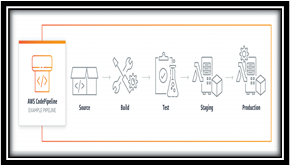
\includegraphics[width=10cm]{./Imagenes/img1.png}
  
    \label{rg4}
    \end{center}
    \end{figure}

\subsection{¿QUÉ ES AZURE DEVOPS?}

    Es una plataforma de SaaS 
    (software como servicio) de Microsoft que nos proporciona una cadena de herramientas DevOps de punto a punto para desarrollar e implementar software. También proporciona alojamiento Git privado ilimitado, compilación en la nube para la integración continua, planificación ágil y administración de versiones 
    para la entrega continua a la nube y en las instalaciones. Incluye amplio soporte IDE.
    \begin{figure}[h]
        \begin{center}
        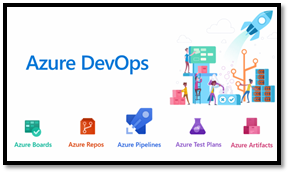
\includegraphics[width=10cm]{./Imagenes/img2.png}
   
        \label{rg4}
        \end{center}
        \end{figure}




\subsection{COMPARATIVA ENTRE AMBOS: VENTAJAS}

Se muestra una comparativa en ventajas entre AWS Codepipeline y Azure DevOps


\begin{figure}[h]
    \begin{center}
    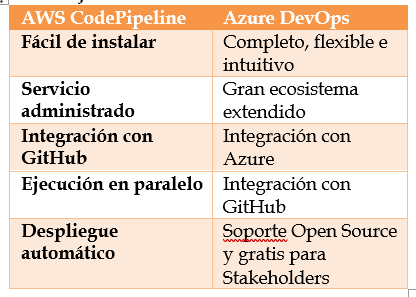
\includegraphics[width=10cm]{./Imagenes/img21.png}
  
    \label{rg5}
    \end{center}
    \end{figure}






\subsection{COMPARATIVA ENTRE AMBOS: DESVENTAJAS}
Se muestra una comparativa en desventajas entre AWS Codepipeline y Azure DevOps
\begin{figure}[h]
    \begin{center}
    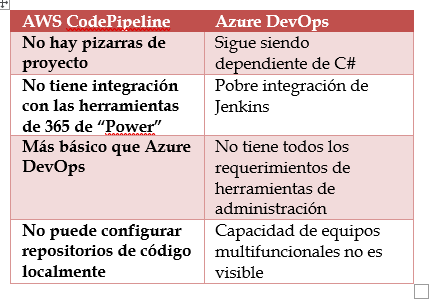
\includegraphics[width=10cm]{./Imagenes/img3.png}
    
    \label{rg5}
    \end{center}
    \end{figure}

\subsection{COMPAÑIAS QUE USAN ESTAS HERRAMIENTAS:}
Se muestran las compañias que utilizan las herramientas.

\begin{figure}[h]
    \begin{center}
    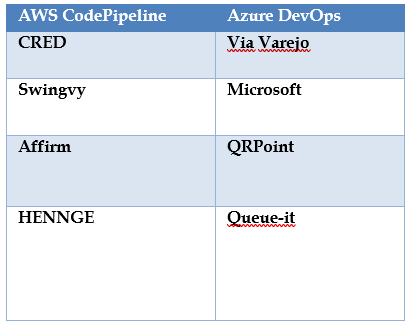
\includegraphics[width=10cm]{./Imagenes/img4.png}
    
    \label{rg6}
    \end{center}
    \end{figure}

\subsection{HERRAMIENTAS QUE PUEDEN SER INTEGRADAS:}
Se muestran herramientas que puede ser integradas en un futuro
\begin{figure}[h]
    \begin{center}
    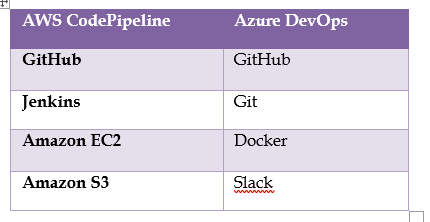
\includegraphics[width=10cm]{./Imagenes/img5.png}
    \caption{Ranorex}
    \label{rg7}
    \end{center}
    \end{figure}
\subsection{ALGUNAS BUENAS ALTERNATIVAS A AMBOS:}


\begin{itemize}
    \item AWS CodeDeploy
    \item Jenkins
    \item AWS CodeBuild
    \item TeamCity
    \item Bamboo

\end{itemize}
\subsection{Google Code Build}

Cloud Build es un servicio que ejecuta tus compilaciones en la infraestructura de Google Cloud Platform. Cloud Build puede importar código fuente de Cloud Storage, Cloud Source Repositories, GitHub o Bitbucket, ejecutar una compilación según tus especificaciones y producir artefactos como contenedores de Docker o archivos de Java. Más información.
Cloud Build ejecuta la compilación como una serie de pasos de compilación, en los que cada uno se ejecuta en un contenedor de Docker. Un paso de la compilación puede todo lo que se puede hacer desde un contenedor, sin importar el entorno. Para realizar tus tareas, puedes usar los pasos de la compilación compatibles que proporciona Cloud Build o escribir tus propios pasos de la compilación.

\subsection{Github Actions}

Las acciones de GitHub te ayudan a 
automatizar tareas dentro del ciclo de vida de 
tu desarrollo de software. Las acciones de GitHub 
están controladas por eventos, lo que significa que puede
 ejecutar una serie de comandos después de que se haya producido 
 un evento específico. Por ejemplo, cada vez que alguien crea una 
 solicitud de extracción para un repositorio, puede ejecutar
  automáticamente un comando que ejecuta un script de prueba de software.
\section{Conclusiones}
CodePipeLine
\begin{itemize}
    \item CodePipeline es una herramienta de entrega continua e integración continua muy flexible.
    \item Facilita un poco la implementación en el entorno de AWS. Hay una gran disponibilidad de datos no estructurados.
    \item Se usa bastante para gestionar la CI/CD (Integración continua e integración delivery)
    
\end{itemize}
Azure DevOps
\begin{itemize}
    \item Es muy fácil de configurar y usar si tiene alguna experiencia con procesos ágiles.     \item Facilita un poco la implementación en el entorno de AWS. Hay una gran disponibilidad de datos no estructurados.
    \item Las barreras de entrada iniciales son extremadamente bajas, ya que los primeros 5 usuarios pueden aprovechar la herramienta de forma gratuita. Encontré la característica / funcionalidad general más fácil de usar y más accesible que herramientas similares. 
    \item Si ya es un usuario de git, esto se integra directamente con los repositorios de git, lo que facilita la transición. 
    \item La herramienta también está integrada con muchos otros productos de Microsoft, por lo que si tiene una tienda centrada en Microsoft, puede aprovechar el ecosistema más amplio.
\end{itemize}

\section{Recomendaciones}
Aquí una serie de aspectos a tener en cuenta al momento de elegir una herramienta para la gestión de prueba
\begin{itemize}
    \item	La categoría de defectos
    \item	El lenguaje de programación y entorno de desarrollo
    \item	El proceso de configuración y gestión de datos de prueba
    \item	El control de versiones y CI (Integración Contínua)
    \item	Los reportes
    \item	Las plataformas compatibles y etiquetado

\end{itemize}

\begin{thebibliography}{XXX0000}

\bibitem - Espinosa, S. G. (2016 de 03 de 1). Personalización del proceso de pruebas unitarias empleando la herramienta NUnit. Obtenido de serie cientifica: https://publicaciones.uci.cu/index.php/serie/article/view/811
\bibitem - Ríos, J. R. (23 de 09 de 2016). Evaluación de los Frameworks en el Desarrollo de Aplicaciones Web con Python. Obtenido de revistas unla: http://revistas.unla.edu.ar/software/article/view/1149
\bibitem - sierra, f. (01 de marzo de 2017). Estudio y análisis de los framework en php basados en el modelo vista controlador para el desarrollo de software orientado a la web. Obtenido de Investigación y desarrollo en TIC: http://revistas.unisimon.edu.co/index.php/identic/article/view/2480
\bibitem - sierra, f. (01 de marzo de 2017). Estudio y análisis de los framework en php basados en el modelo vista controlador para el desarrollo de software orientado a la web. Obtenido de Investigación y desarrollo en TIC: http://revistas.unisimon.edu.co/index.php/identic/article/view/2480 
\bibitem - Paloma Díaz, Susana Montero, Ignacio Aedo. (2005). Ingeniería de la web y patrones de diseño.
\bibitem - Villón Moreno, M. S. (abril de 2019). Plataforma tecnológica para contribuir a la planeación urbana en la ciudad de Guayaquil dirigido a la transportación enfocado al diseño de pruebas que permitan la verificación y validación del software usando herramientas de pruebas ágiles. Obtenido de repositorio institucional de la universidad de guayaquil: http://repositorio.ug.edu.ec/handle/redug/39670
\bibitem - Paloma D´ıaz, Susana Montero, Ignacio Aedo. (2005). Ingenier´ıa de la web
\bibitem - https://www.trustradius.com/products/aws-codepipeline/reviews
\bibitem - https://www.trustradius.com/compare-products/aws-codepipeline-vs-azure-devops
\bibitem - https://www.infoworld.com/article/3271126/what-is-cicd-continuous-integration-and-continuous-delivery-explained.html

\end{thebibliography}
\end{document}